\documentclass[a4paper,12pt]{report}
\usepackage[utf8]{inputenc}
\usepackage{titlesec}
\usepackage{nameref}
\usepackage{tabularx}
\usepackage{amsmath}
\usepackage{amsfonts}
\usepackage{amssymb}
\usepackage{graphicx}

\titleformat{\chapter}[display]
  {\normalfont\bfseries}{}{0pt}{\huge}

% Title Page
\title{{\bf berry} suite of programs\\
\large Documentation \\
v.0.3.2}
\author{Ricardo Mendes Ribeiro}
\date{\today}
\makeindex


\begin{document}
\begin{titlepage}
 \begin{center}
 
\includegraphics[scale=0.3,keepaspectratio=true]{figures/BerryLogo.png}
% BerryLogo.png: 2310x2310 px, 300dpi, 19.56x19.56 cm, bb=0 0 554 554
\vspace*{2cm}

  \begin{Huge}{\bf berry} suite of programs  \end{Huge}
  \vspace*{1cm}

 \begin{LARGE}Documentation              \end{LARGE}
  \vspace*{1cm}

\begin{Huge}v.0.3.2\end{Huge}
  \vspace*{0.5cm}

\today

 \end{center}
\end{titlepage}

\tableofcontents

\chapter{Introduction}\label{ch:introduction}

 This guide gives a general introduction to the \textbf{berry} suite of programs, including instalation and running.
 An introduction to the basics of electronic structure calculations is given, in the context of this suite.

 All programs of this package are in python 3.

The package contains the python scripts:
\begin{itemize}
 \item preprocessing.py
 \item generatewfc.py
 \item dotproduct.py
 \item compara.py
 \item interpolation.py
 \item basisrotation.py
 \item r2k.py
 \item berryConnection.py
 \item berryCurvature.py
 \item condutivity.py
 \item shg.py
\end{itemize}\medskip

and the auxiliary and visualization scripts:
\begin{itemize}
 \item draw2D\_machine.py
 \item draw2D\_corrected.py
 \item drawberry.py
 \item drawcurvature.py
 \item emailSender.py
 \item viewdata.py
 \item viewdot1.py
 \item viewdot.py
 \item vieweigenvalues.py
 \item viewneighbors.py
 \item viewoccupations.py
 \item viewr.py
\end{itemize}\medskip

Also with some subroutines (depend on the other scripts):
\begin{itemize}
 \item headerfooter.py
 \item contatempo.py
 \item parser.py
 \item loaddata.py
 \item dft.py
 \item comutator.py
 \item write\_k\_points.py
 \item NestablePool.py
\end{itemize}

It is likely that some of these scripts will be merged with others
while new ones will appear due to new functionalities.







\section{People}

The \textbf{berry} suite is coordinated by Ricardo Mendes Ribeiro (University of Minho and INL, Braga, Portugal),
which is also the main developer.\medskip

Other contributors include
\begin{itemize}
 \item Ícaro Jael Moura (Fortaleza, Brasil) for the exploratory work and testing;
 \item Irving Leander Reascos Valencia (Braga, Portugal) for improving the performance and AI work;
 \item Fábio Carneiro for the parallelization of the python code and its performance;
 \item Nuno Castro (LIP-Minho, Braga, Portugal) for coordinating AI work;
 \item Gonçalo Ventura (Porto, Portugal) for the equations for non-linear optical properties calculated from the Berry connections;
 \item Afonso Duarte Ribeiro, author of the logo.
\end{itemize}


\section{Contacts}

The web site for the \textbf{berry} suite is\medskip

https://ricardoribeiro-2020.github.io/berry/\medskip

All files for instalation can be found there.

There is still no mailling list for reporting bugs or other questions, but an email can be sent to
ricardo.ribeiro@physics.org


\section{Electronic structure calculations basics}

\subsection*{Crystal}
A crystal is defined by its translational symmetry.
A set of atoms, a pattern, is replicated all over space in one, two or three dimensions.
It forms a crystal \emph{lattice}.

Here we will deal only with 2D materials, so the pattern, which is called \emph{unit cell},
is repeated in two dimensions, in a plane.

\begin{figure}
 \centering
 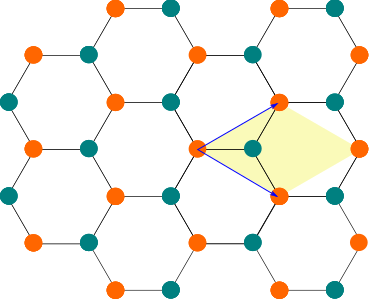
\includegraphics[scale=0.5,keepaspectratio=true]{figures/unitcell_honeycomb.png}
 \caption{Example of a unit cell in a two dimensional material, with hexagonal symmetry.
 The yellow shadow represents the unit cell and the two blue vectors represent the lattice vectors.}
 \label{fig:unitcell}
\end{figure}

The unit cell is defined by three vectors (two in 2D) $\pmb{a}_1$, $\pmb{a}_2$ and $\pmb{a}_3$,
in position space (the real space).
One can go from one unit cell to any other one by aplying the translation
\begin{equation}
 \pmb{R} = n_1\pmb{a}_1 + n_2\pmb{a}_2 + n_3\pmb{a}_3
\end{equation}
where $n_1$, $n_2$ and $n_3$ are integers, and $\pmb{R}$ is called the lattice vector.

A Fourier transform of this periodic pattern gives another periodic pattern in the so-called
\emph{reciprocal space} or momentum space.
This new periodicity is defined by the reciprocal vectors:
\begin{equation*}
 \pmb{b}_1 = 2\pi\dfrac{\pmb{a}_2\times\pmb{a}_3}{\pmb{a}_1\cdot (\pmb{a}_2\times\pmb{a}_3)};\hspace*{1cm}
 \pmb{b}_2 = 2\pi\dfrac{\pmb{a}_3\times\pmb{a}_1}{\pmb{a}_1\cdot (\pmb{a}_2\times\pmb{a}_3)};\hspace*{1cm}
 \pmb{b}_3 = 2\pi\dfrac{\pmb{a}_1\times\pmb{a}_2}{\pmb{a}_1\cdot (\pmb{a}_2\times\pmb{a}_3)}
\end{equation*}

\subsection*{Electrons in a crystal}

Electrons in a crystal can be described by the solutions to time independent Schr\"odinger equation:
\begin{equation}\label{eq:Schrodinger}
 H_{\pmb{k}}\psi_{\pmb{k},s}(\pmb{r}) = E_{\pmb{k},s}\psi_{\pmb{k},s}(\pmb{r})
\end{equation}
where $H_{\pmb{k}}$ is the hamiltonean of the system, which has the periodicity of the crystal lattice,
and is a function of the momentum $\pmb{k}$.
For each $\pmb{k}$ we have an equation \ref{eq:Schrodinger} that gives a (infinite) set of solutions,
which are labeled by the letter $s$.

The eigenvalues are the energies $E_{\pmb{k},s}$ and the respective eigenvectors are the wavefunctions
$\psi_{\pmb{k},s}(\pmb{r})$.

For a periodic material, the solutions to equation \ref{eq:Schrodinger} are given by Bloch's theorem:
\begin{equation}
 \psi_{\pmb{k}s}(\pmb{r}) = e^{i\pmb{k}\cdot\pmb{r}}u_{\pmb{k}s}(\pmb{r})
\end{equation}
with
\begin{equation}
 u_{\pmb{k}s}(\pmb{r}) = u_{\pmb{k}s}(\pmb{r} + \pmb{R})
\end{equation}
and $\pmb{k}$ is a point within the Brillouin Zone (BZ) and $s$ numbers the bands.
$\pmb{R}$ is the lattice vector.

$u_{\pmb{k}s}(\pmb{r})$ is called the Bloch factor and $e^{i\pmb{k}\cdot\pmb{r}}$
is called the Bloch phase factor.


\subsection*{Bands}

In the previous subsection the solutions of the Schr\"odinger equation were ordered by a \emph{band} index $s$.
In practice, the eigenvectors and eigenvalues are ordered in increasing energy, so that $E_{\pmb{k},0}$ is
the lowest energy solution of equation \ref{eq:Schrodinger}, $E_{\pmb{k},1}$ is the second lowest energy solution,
and so on.

Actually, there are a number of property calculations where it is necessary to use the set of eigenvectors
and eigenvalues that form a band as an entity in which mathematical operators must be applied
(the gradient in momentum space, for instance).
The Berry connection is an example.
The Berry connection is defined as:
\begin{equation}\label{eq:berry}
 \pmb{\xi}_{\pmb{k}ss'} = i\langle u_{\pmb{k}s}|\nabla_{\pmb{k}} u_{\pmb{k}s'} \rangle
                          = \dfrac{i}{v_C}\int_{uc} d^3\pmb{r}u_{\pmb{k}s}^*(\pmb{r})
                          \nabla_{\pmb{k}} u_{\pmb{k}s'}(\pmb{r})
\end{equation}
where $v_C$ is the volume of the unit cell and $uc$ stands for unit cell.

But the ordering (and grouping) of eigenstates by energy fails to give an usable entity for a gradient calculation,
because it frequently has discontinuities, i.e. is non-analytic.
\begin{figure}
 \centering
 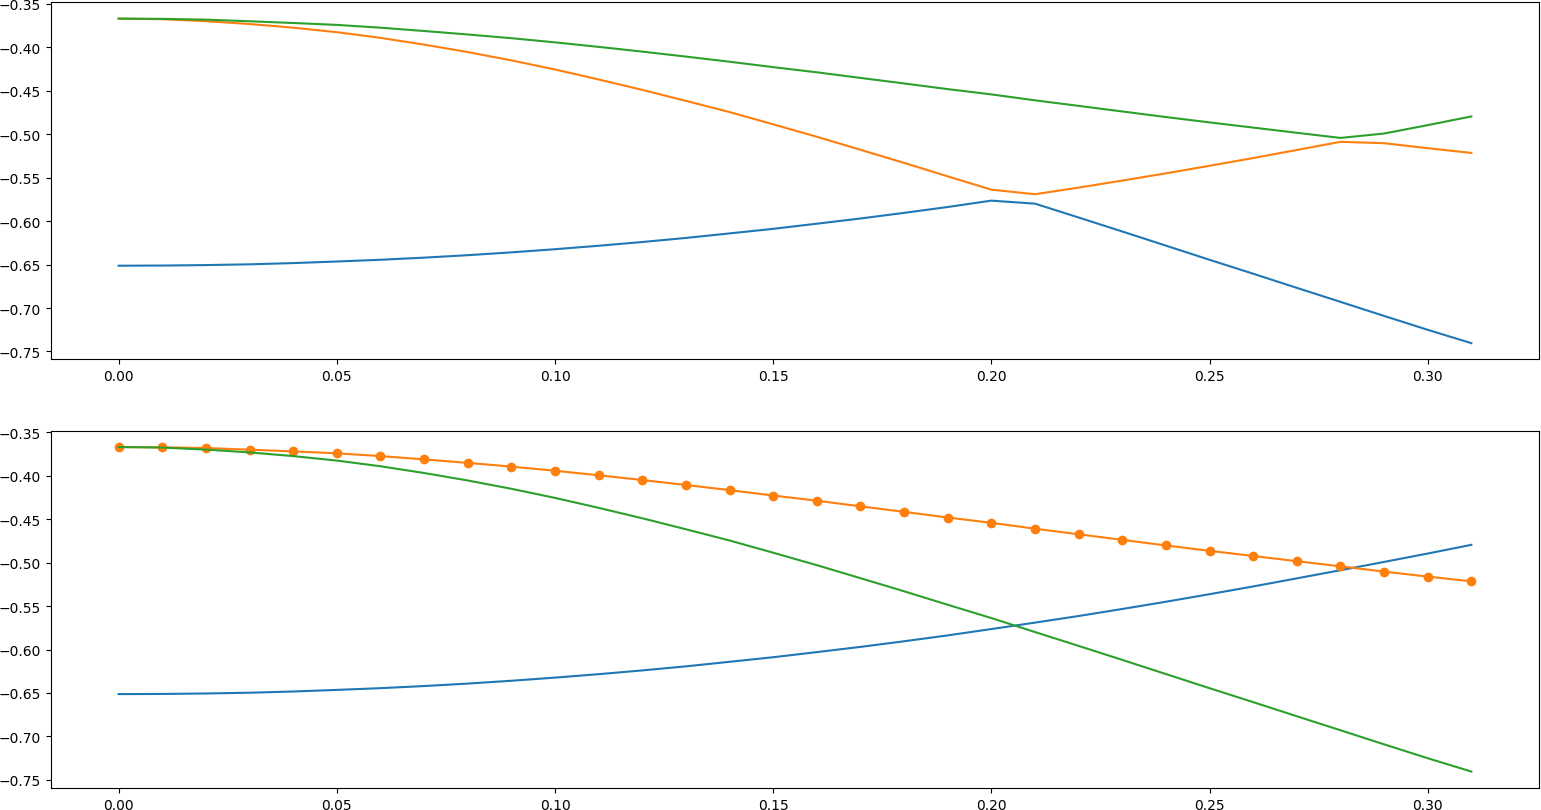
\includegraphics[scale=0.3,keepaspectratio=true]{figures/order_bands1D.png}
 % order_bands1D.png: 1541x810 px, 100dpi, 39.14x20.57 cm, bb=0 0 1110 583
 \caption{Example of electronic bands in one dimension.
 Different colors indicate different bands.
 Top: the bands according to the DFT output, that is, ordered by energy.
 Bottom: the bands according to continuity of the Bloch factors.
 The dots on the orange curve in the bottom figure indicate the positions of the k point sampling.}
 \label{fig:orderbands}
\end{figure}
Figure \ref{fig:orderbands} ilustrates the problem.
Where actual bands cross, the simple energy ordering cannot keep with the right band and jumps to another,
leading in fact to a discontinuity.

In order to be able to apply a gradient in momentum space we need to have the eigenstates ordered and grouped
in such a way that analycity is guaranteed.
That is the first goal of this suite of programs.



\subsection*{Band crossings}\label{ssec:bandcrossings}

It is clear that the problem of classifying the eigenstates by bands where analycity applies is
only problematic at degeneracies i.e. band crossings.

There, any linear combination of eigenstates is also an eigenstate.

Lets consider two bands $A$ and $B$, crossing at point $k$.
The eigenstates of $A$ are continuous at the left of $k$ and at the right, and the same is true for eigenstates of $B$.
But not necessarily at $k$.
Supppose that $\psi_A$ would be the wavefunction at $k$ that would have continuity in band $A$
and $\psi_B$ for band $B$. Of course, $\psi_A$ and $\psi_B$ have the same eigenvalue.

But the numerical process of solving the Schr\"odinger equation at point $k$ can give any result of the form
\begin{align}
 \psi_1 &= a\psi_A + b\psi_B \\
 \psi_2 &= a'\psi_A + b'\psi_B
\end{align}
as long as $\psi_1$ and $\psi_2$ are orthogonal (the coeficcients have to be such that they assure orthogonality).
Of course, these wavefunctions are not continuous with $A$ or $B$, in general.

There are two ways to workaround this problem and restore analycity.
One is to interpolate the wavefunction at $k$ using the closest eigenstates of band $A$ and then the ones of band $B$.
The other is to apply an unitary transformation.

\paragraph*{Interpolation}
Assume that $\psi_A^-$ and $\psi_A^+$ are the wavefunctions immediatly at left and right of $k$ that belong to band $A$,
and $\psi_B^-$ and $\psi_B^+$ are the same for band $B$.
Wavefunctions of bands $A$ and $B$ in the same point in momentum space are orthogonal, so $\psi_A^- \perp \psi_B^-$
and $\psi_A^+ \perp \psi_B^+$.
Even a simple interpolation
\begin{align}
 \psi_A &= \dfrac{1}{2}\left( \psi_A^- + \psi_A^+\right) \\
 \psi_B &= \dfrac{1}{2}\left( \psi_B^- + \psi_B^+\right)
\end{align}
will lead to $\psi_A \perp \psi_B$ and restore analycity within the numerical precision,
since $\psi_A^-$ and $\psi_A^+$ are very close and continuous,
and the same for $\psi_B^-$ and $\psi_B^+$.
This results from the continuity of the hamiltonean in momentum space.


\paragraph*{Unitary transformation}
The most frequent way of restoring analycity is to apply an unitary transformation
\begin{equation}
 \left[ \begin{matrix}
  \psi_A\\\psi_B
 \end{matrix}\right] = U
 \left[ \begin{matrix}
  \psi_1\\\psi_2
 \end{matrix}\right]
\end{equation}
where $U$ is choosen in such a way as to 'iron out' the nonanalytic behaviour at $k$.
In practice, this is done by minimizing the difference betwenn $\psi_A$ and both $\psi_A^-$ and $\psi_A^+$,
and the same for $\psi_B$ relative to $\psi_B^-$ and $\psi_B^+$.




\chapter{Instalation}

\section{Download}
The github packages should be downloaded from\medskip

 https://github.com/ricardoribeiro-2020/berry/archive/master.zip\medskip

unziped in the directory where the instalation is to be done and the directory structure kept.

With this, each python script of the suite should run, giving the full path to the script.

\section{Requirements}

This software uses python3 with the following libraries, that have to be installed
(most of these should already be there by default):
\begin{itemize}
 \item numpy
 \item sys
 \item time
 \item joblib
 \item math
 \item os
 \item findiff
 \item matplotlib.pyplot
 \item mpl\_toolkits.mplot3d
 \item xml.etree.ElementTree
\end{itemize}


This version of \textbf{berry} only supports the DFT package {\sc Quantum Espresso}, version v.6.6 or higher.

So a working {\sc Quantum Espresso} instalation has to be in the system, and must be in the \$PATH.

\section{Running}\label{sec:running}

 To run, first one has to create a working directory where the results will be saved,
 and inside it create a directory called \emph{dft}.

 Inside \emph{dft} should go the pseudopotential files for the atomic species of the dft calculation
and the file \emph{scf.in} with the details of the scf run.
You can use another name for the file, but then you have to add a line in the input file of
the script \textbf{preprocessing.py} to change the default (see section \nameref{sec:preprocessing}).

 This \emph{scf.in} file has to be a {\sc Quantum Espresso} scf run file;
 this is the only one implemented so far.

 Create an input file (as described in chapter \nameref{ch:workflow}, section \nameref{sec:preprocessing})
 in the working directory.

 All the scripts should be run from the working directory, using the full path to the python scripts.

\paragraph{Sequence} of programs to run should be the following:
\begin{verbatim}
 preprocessing.py   inputfile
 generatewfc.py
 dotproduct.py
 compara.py [k-point]
 interpolation.py [band] or basisrotation.py [band]
 r2k.py  band1 [band2]
 berryConnection.py  band1 [band2]
 berryCurvature.py   band1 [band2]
 condutivity.py   band1 band2 [inputfile]
 shg.py   band1 band2 [inputfile]
\end{verbatim}
In brackets are optional parameters.




\chapter{Workflow}\label{ch:workflow}

\section{Preprocessing}\label{sec:preprocessing}
 After creating the files and directories mentioned in section \nameref{sec:running}, the next thing is
 to run the script \textbf{preprocessing.py}, which will do the following:
 \begin{enumerate}
  \item Reads file with the description of the run wanted.
  \item Runs the scf calculation using {\sc Quantum Espresso}, if it has not ran before.
  \item Generates an nscf input file according to the input data of the run and runs an nscf calculation,
  using {\sc Quantum Espresso}, if it has not ran before.
  \item Reads data from the nscf calculation and saves to a file.
  \item Makes several simple calculations that will be used afterwards in other scripts, and save them to several files.
 \end{enumerate}

 An input file for the berry run has to be created in the working directory with several parameters.
The minimum parameters needed are:
\begin{itemize}
 \item origin of k-points (k0)
 \item number of k-points in each direction (nkx, nky, nkz)
 \item step of the k-points (step)
 \item number of bands to be calculated (nbnd)
\end{itemize}

An example of the minimum input file is shown in figure \ref{code:inputfile}.
A full list of the parameters that are accepted with the respective defaults (if any)
is shown in table \ref{tab:variables_preprocessing}.
There is a unique reference number that is attributed when running \textbf{preprocessing.py},
that can be changed in the input file, but it not recomendable, because it is too easy to forget
to change that variable in the input file and attribute the same value for different runs.

\begin{figure}[h]
 \centering\caption{Example of input file for \textbf{preprocessing.py}.}
\begin{verbatim}
  k0 0.00 0.00 0.00
  nkx 100
  nky 100
  nkz 1
  step 0.005
  nbnd 8
\end{verbatim}
\label{code:inputfile}
\end{figure}



\begin{table}[h]
 \centering
 \caption{List of variables for the input file of \textbf{preprocessing.py}.}

 \begin{tabularx}{\textwidth}{Xl}
 \textbf{Role of keyword}  & \textbf{Variable (and defaults)}\\
\hline
 origin of k-points  & k0 \\
 number of k-points in each direction  & nkx, nky, nkz \\
 step of the k-points  & step \\
 number of bands to be calculated  & nbnd \\
 \hline
 number of processors  & npr = 1 \\
 dft directory  & dftdirectory = 'dft/' \\
 scf file name  &     name\_scf = 'scf.in' \\
 directory where wavefunctions will be saved  &     wfcdirectory = 'wfc/' \\
 point in real space where all phases match  & point = 1.178097 \\
 software for DFT  &  program = 'QE' \\
 Unique reference of run & refname = date and time \\
%  DFT prefix  & prefix = '' \\
%  DFT output directory & outdir = ''\\
 \hline
\end{tabularx}
 \label{tab:variables_preprocessing}
\end{table}




\newpage
The script \textbf{preprocessing.py} creates the files:
\begin{itemize}
 \item \emph{phase.npy}
 \item \emph{neighbors.npy}
 \item \emph{eigenvalues.npy}
 \item \emph{occupations.npy}
 \item \emph{positions.npy}
 \item \emph{kpoints.npy}
 \item \emph{nktoijl.npy}
 \item \emph{ijltonk.npy}
\end{itemize}
and \emph{datafile.npy} which is the main data file.

File \emph{neighbors.npy} lists the neighbors of each k-point
(which neighbors to consider may be an input parameter in the future).

File \emph{phase.npy} saves for each (k,r) the phase factor of the Bloch functions.

This finishes the preparatory phase.

\section{Extraction of wavefunctions}

The next step is to extract the wavefunctions from the format used in the DFT package
(in this case it is {\sc Quantum Espresso}),
make them coherent and save them in a format adequate for the \textbf{berry} suite.

The script that does this job is \textbf{generatewfc.py}.

It uses the package wfck2r.x of the {\sc Quantum Espresso} suite to extract and save the wavefunctions
from the original format to a text file, in position space, one for each k-point and band.

Then a point in position space is choosen (see table \ref{tab:variables_preprocessing}),
away from points of high symmetry, and all wavefunctions
are multiplied by a phase such that at that point all wavefunctions have zero phase.

Then the wavefunctions are saved in the directory choosen to save them
(see table \ref{tab:variables_preprocessing}; default is \emph{./wfc/}),
and the files will be named in the form \emph{k0**b0XX.wfc} where ** is replaced by the number of the k point
and \emph{XX} is replaced by the number of the band.
Bands are as given by the DFT software i.e. ordered by energy, and the lowest energy band is numbered zero and so on.


\section{Dot product}

\textbf{dotproduct.py} reads the wavefunctions saved in directory \emph{./wfc/},
removes the phase factor of the Bloch functions, and calculates the dot product
of the Bloch factors of the neighboring k points.

The neighboring k points are the four nearest neighbors, as determined in the preprocessing
and saved in file \emph{neighbors.npy}.

In the end we get two files \emph{dpc.npy} and \emph{dp.npy}:
\begin{itemize}
 \item \emph{dpc.npy} contains for each pair of k-points and bands the dot product of the wavefunctions
 \item \emph{dp.npy} contains the modulus of \emph{dpc.npy}
\end{itemize}


\section{Establishing the bands}
Find which eigenvalues/eigenfunctions have continuity, by running program \textbf{compara.py}.

This program reads the dot product file \emph{dp.dat} and uses it to check continuity.

 It retrieves two files:
 \begin{description}
   \item[\emph{bandsfinal.npy}] stores an array bandsfinal[k,b] = number of band that is continuous to band b
   \item[\emph{signalfinal.npy}] signalfinal[k,b] equals -1 if there is an inconsistency at
   that k-point or a number $\ge0$
  giving the number of times it found a continuity. The larger the value, the better.
 \end{description}

 \textbf{compara.py} may need to be run several times until the results are good.
 Not that it improves as the number of trials increases, but the starting point
 (which is choosen randomly, but can be specified explicitly as an input parameter)
 may simply be a better one to find the continuities.


\section{Interpolation}
 As discussed in subsection \ref{ssec:bandcrossings} of the \nameref{ch:introduction},
 there may be a few k points where there are actual discontinuities and so need to restore analitycity.

 For this, \textbf{interpolation.py} should be run, which uses the interpolation method described in that subsection.

 The interpolation done by \textbf{interpolation.py} is not a simple mean value but a polinomial interpolation
 that uses up to six surrounding k points to do the job.

 It will create new interpolated wavefunctions with extension \emph{.wfc1}, that will be used in subsequent calculations.

 Since you probably just want to interpolate in the bands that are well determined, and argument with the last band number
 is needed.
 \begin{verbatim}
  python3 interpolate.py [band number]
 \end{verbatim}

\section{Basis rotation}
 Instead of the interpolation suggested in the last section, it is more frequent that a basis rotation
 is applied to the wavefunctions in such a way as to maximize continuity.

 For this, \textbf{basisrotation.py} can be run.
 It works like this:
 Consider a point in k-space and two wavefunctions $|\Psi_1\rangle$ and $|\Psi_2\rangle$
 that have been signaled as not continuous to the neighboring wavefunctions $|\Psi_A\rangle$ and $|\Psi_B\rangle$
 that belong to band $A$ and band $B$, respectively.

 We will apply an unitary transformation
 \begin{align*}
  |\Psi_A'\rangle &= a_1|\Psi_1\rangle + a2|\Psi_2\rangle \\
  |\Psi_B'\rangle &= b_1|\Psi_1\rangle + b2|\Psi_2\rangle
 \end{align*}
 where we have the restrictions due to orthonormalization:
 \begin{align*}
  a_1a_1^* + a_2a_2^* &= 1\\
  b_1b_1^* + b_2b_2^* &= 1\\
  a_1^*b_1 + a_2^*b_2 &= 0
 \end{align*}

 Then we want this transformation to be such that maximizes continuity to bands $A$ and $B$, so we want
 the dot products $\langle \Psi_A|\Psi_A'\rangle $ and $\langle \Psi_B|\Psi_B'\rangle $ to be close to $1$,
 which is the maximum they can be.

 We look for the set $a_1, a_2, b_1, b_2$ that give
 \begin{align*}
  \max \langle \Psi_A|\Psi_A'\rangle &= \max \left( \langle \Psi_A|\Psi_1\rangle a_1 + \langle \Psi_A|\Psi_2\rangle a_2\right) \\
  \max \langle \Psi_B|\Psi_B'\rangle &= \max \left( \langle \Psi_B|\Psi_1\rangle b_1 + \langle \Psi_B|\Psi_2\rangle b_2\right)
 \end{align*}



 It will create new wavefunctions with extension \emph{.wfc1}, that will be used in subsequent calculations.

 Since you probably just want to interpolate in the bands that are well determined, and argument with the last band number
 is needed.
 \begin{verbatim}
  python3 basisrotation.py [band number]
 \end{verbatim}

\section{Convert wavefunctions to k space}

With the bands right, now proceeds to calculate the wavefunctions in k-space and their gradients.

For that, run \textbf{r2k.py} with one or two arguments:
\begin{itemize}
 \item If one, will calculate from band 0 to the value inputed.
 \item If two, will calculate for the set of bands between the two values, inclusive.
\end{itemize}

 Will save the wavefunctions of each band in a compressed file \emph{wfcpos\#.gz} where \# = number of band.
 This will be a dictionary with a label for each position in real space (from 0 to nr) and for each label
 a numpy array with the complex value of the wavefunction for each k point in momentum space.

 Will save the gradients of each band in a compressed file \emph{wfcgra\#.gz} where \# = number of band.

\section{Calculation of the Berry connections and curvatures}

The Berry connections (equation \ref{eq:berry}) are calculated using the script \textbf{berryConnection.py}
and the Berry curvature with \textbf{berryCurvature.py}.

These scrips must have one or two integers as input.

If it is just one, the scripts will calculate for all combinations of bands from the first up to the
number given as input.

If two integers are given, they will only calculate the Berry connection (or curvature) for that pair of bands.


\section{Optical conductivity and second harmonic generation}
Calculate the linear condutivity by running \textbf{condutivity.py}
and the second harmonic condutivity by running \textbf{shg.py}.

Both need two or three arguments.

 If there are two:  the first is the last filled band, the second is last empty band.
 If the first argument is negative, it will only consider transitions from one band to the other, while if it is positive it will consider all bands below the first value and all the empty bands up to the second value.
 Real part has to be always positive and zero below the gap.

 The third argument, if it exists, is the name of an input file that should have the values wanted for\medskip

\begin{tabularx}{\textwidth}{Xl}
 enermax  2.5            & Maximum energy (Ry)\\
 enerstep  0.001         & Energy step (Ry)\\
 broadning  0.01j        & energy broadning (Ry) \\
\end{tabularx}
\medskip

(these are the default values, if there is no input file)







\chapter{Glossary}

This glossary indicates the meaning of the variables used in the suite \textbf{berry}.
\vspace{0.5cm}

\begin{tabularx}{\textwidth}{Xl}
 npr            & Number of processors for the run \\

 nkx            & Number of k-points in the x direction \\
 nky            & Number of k-points in the y direction \\
 nkz            & Number of k-points in the z direction \\
 nks            & Total number of k-points \\

 nr1            & Number of points of wfc in real space x direction \\
 nr2            & Number of points of wfc in real space y direction \\
 nr3            & Number of points of wfc in real space z direction \\
 nr             & Total number of points of wfc in real space \\

 k0             & Initial k-point (coordinates) (2pi/bohr) \\
 step           & Step between k-points (2pi/bohr) \\
\end{tabularx}
\vspace{0.5cm}

\begin{tabularx}{\textwidth}{Xl}
 dftdirectory   & Directory of DFT files \\
 name\_scf       & Name of scf file (without suffix) \\
 name\_nscf      & Name of nscf file (without suffix) \\
 wfcdirectory   & Directory for the wfc files \\
 prefix         & Prefix of the DFT QE calculations \\
 outdir         & Directory for DFT saved files \\
 dftdatafile    & Path to DFT file with data of the run \\
 berrypath      & Path of BERRY files \\
\end{tabularx}
\vspace{0.5cm}

\begin{tabularx}{\textwidth}{Xl}
 a1             & First lattice vector in real space (bohr) \\
 a2             & Second lattice vector in real space (bohr) \\
 a3             & Third lattice vector in real space (bohr) \\

 b1             & First lattice vector in reciprocal space ($2\pi$/bohr) \\
 b2             & Second lattice vector in reciprocal space ($2\pi$/bohr) \\
 b3             & Third lattice vector in reciprocal space ($2\pi$/bohr) \\
\end{tabularx}
\vspace{0.5cm}

\hspace*{-2cm}\begin{tabularx}{\textwidth}{ll}
 nbnd           & Number of bands \\

 eigenvalues    & Array with all eigenvalues of the calculation (Ry) \\
 occupations    & Array with all occupations of the calculation \\

 phase[i,nk]    & Array with exp(1j*(kpoints[nk,0]*r[i,0] + kpoints[nk,1]*r[i,1] + kpoints[nk,2]*r[i,2])) \\
 kpoints[nk,2]  & Array with coordinates of all k-points ($2\pi$/bohr) \\
 r[i,2]         & Array with coordinates of all points of space (bohr) \\

 neig[nk,3]     & Array with number of the four k-points around nk \\
\end{tabularx}





\end{document}
